\documentclass[border=5mm]{standalone}
\usepackage{tikz} % Required for TikZ drawings
\usepackage{xcolor} % Required for defining custom colors
\usetikzlibrary{positioning, backgrounds, fit}
\usetikzlibrary{shapes.geometric, arrows}
\tikzstyle{startstop} = [rectangle, rounded corners, minimum width=3cm, minimum height=1cm, text centered, draw black, fill=red!30]



% Define colors
\definecolor{safetyColor}{HTML}{0d6a82}
\definecolor{biodiversitycolor}{HTML}{fb4d3d}
\definecolor{3dmodelColor}{HTML}{345995}
\definecolor{applicationColor}{HTML}{e7901a}
\definecolor{backgroundColor}{HTML}{2a9d8f}
\definecolor{challengeColor}{HTML}{606c38}
\definecolor{applicationBackground}{HTML}{ffb703}

% Style definitions
\tikzset{
 base node/.style={
%  rounded corners=3pt,
                        % draw=gray!40,
                        % fill=white,
                        % drop shadow,
 minimum width=1cm,
 align=center,
 minimum height=0.75cm,
 inner sep=5pt
 },
 category box/.style={
 rectangle,
 rounded corners,
 draw=black,
%  fill=gray!5,
 inner sep=5pt
 },
 arrow/.style={
 -latex,
 ultra thick,
 opacity=0.9
 },
 3dmodels/.style={base node, fill=white, draw=black},
 biodiversity/.style={base node, fill=biodiversitycolor!5, draw=biodiversitycolor},
 safety/.style={base node, fill=safetyColor!5, draw=safetyColor},
 applications/.style={base node, fill=applicationColor!5, draw=applicationColor},
 title/.style={minimum height=0cm, align=center},
 optimized/.style={dashed, draw=safetyColor, thick},
 optimizedbox/.style={optimized, fill=safetyColor!5}
}


\begin{document}
\begin{tikzpicture}

	\draw[white, fill=white] (9.7, 0) rectangle (12.5, 5);
	\node[anchor=south west,inner sep=0] (image) at (0,0) {
		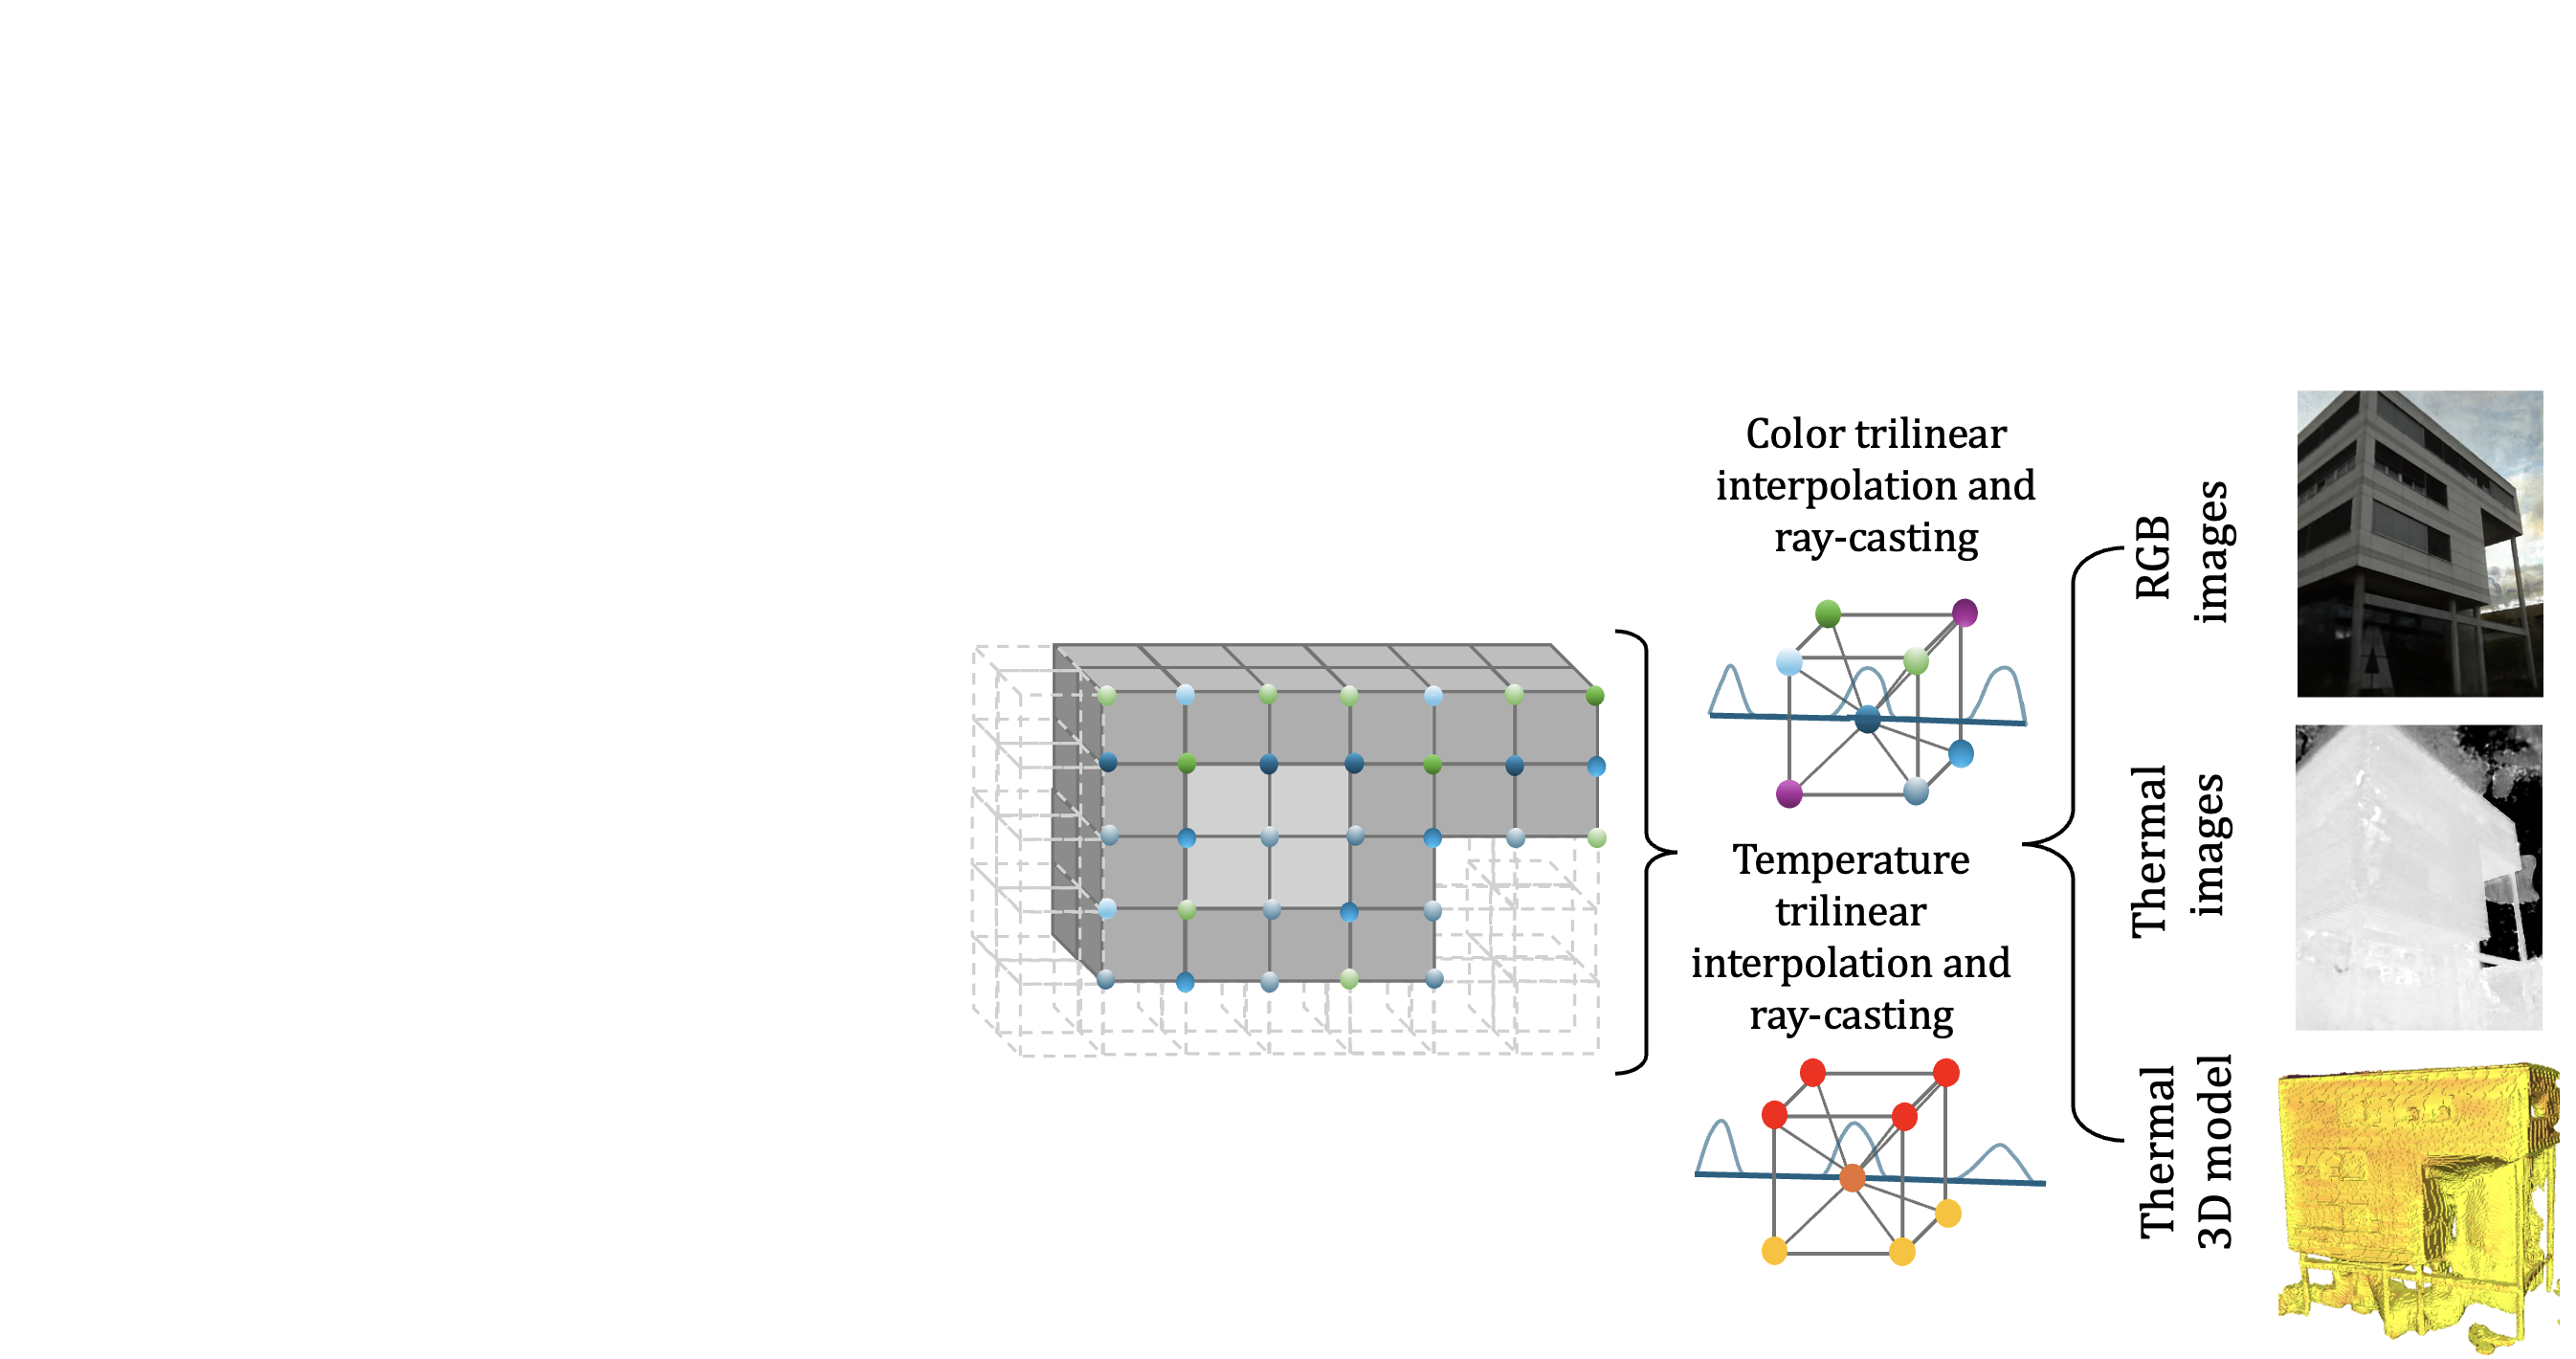
\includegraphics[width=\textwidth]{thermoxels_pipeline.png}
	};

	\node[applications] (pose) at (3.5, 2.5) {Poses};
	\node[inner sep=0] (rgb) at (6, 4.75) {
		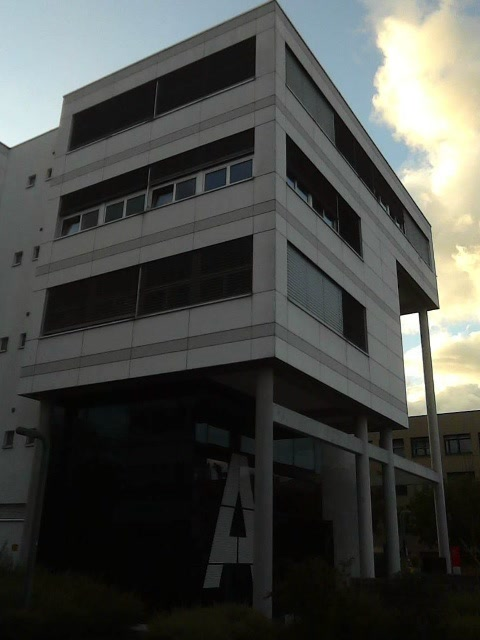
\includegraphics[width=0.1\textwidth]{dataset_building-a-spring_rgb.jpeg}
	};
	\node[inner sep=0] (thermal) at (6,0) {
		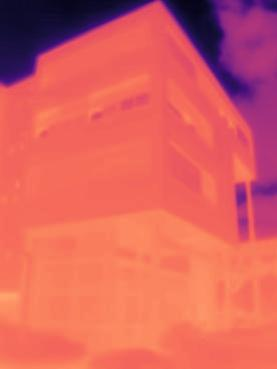
\includegraphics[width=0.1\textwidth]{dataset_building-a-spring_thermal.jpeg}
	};

	\draw[-latex] (pose) -- (7.5,3.5);
	\draw[-latex] (pose) -- (7.5,3);
	\draw[-latex] (pose) -- (7.5,2.5);
	\draw[-latex] (pose) -- (7.5,2);
	\draw[-latex] (pose) -- (7.5,1.5);

	\draw[-latex, color=red] (pose) -- (7.5,3.6);
	\draw[-latex, color=red] (pose) -- (7.5,3.1);
	\draw[-latex, color=red] (pose) -- (7.5,2.6);
	\draw[-latex, color=red] (pose) -- (7.5,2.1);
	\draw[-latex, color=red] (pose) -- (7.5,1.6);

	\draw[-latex] (9, 4.5) -- (9, 4.75) -- (rgb);
	\draw[-latex] (9, 0.25) -- (9, 0) -- (thermal);
	\draw[-latex] (rgb) -- (6, 3.5);
	\draw[-latex] (thermal) -- (6, 1.25);

	%Draw a white rectangle
	% \draw[white, fill=white] (9.5, 2) rectangle (12.5, 2.5);

\end{tikzpicture}

\end{document}
